% Shared standalone design for the editable figure reconstructions.
\documentclass[tikz,border=5pt,10pt]{standalone}
\usepackage[T1]{fontenc}
\usepackage[utf8]{inputenc}
\usepackage{newpxtext,newpxmath}
\usepackage[scaled=.94]{sourcesanspro}
\usepackage{pgfplots}
\pgfplotsset{compat=1.18}
\usetikzlibrary{arrows.meta,calc,positioning,decorations.pathreplacing,
  decorations.markings,patterns,matrix,shapes.geometric,fit,backgrounds,
  intersections,angles,quotes}
\definecolor{ink}{HTML}{203746}
\definecolor{accent}{HTML}{146C78}
\definecolor{muted}{HTML}{667780}
\definecolor{signalred}{HTML}{B94B44}
\color{ink}
\tikzset{>=Latex,line width=.8pt,
  every node/.style={font=\small},
  axis/.style={->,draw=muted,line width=.5pt},
  guide/.style={draw=muted,dashed,line width=.45pt},
  curve/.style={draw=accent,line width=1pt},
  marker/.style={circle,fill=accent,inner sep=1.5pt},
  labelbox/.style={fill=white,inner sep=2pt}}

\begin{document}
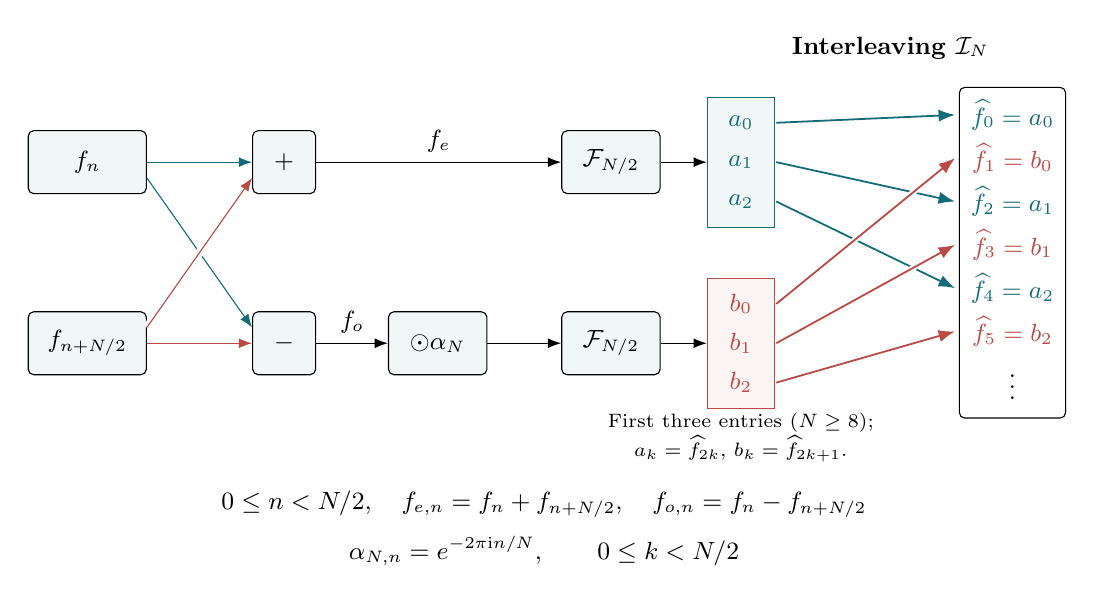
\begin{tikzpicture}[x=1cm,y=1cm,block/.style={draw,rounded corners=2pt,fill=accent!6,minimum width=1.25cm,minimum height=.8cm,align=center},every node/.style={font=\small}]
\node[block,minimum width=1.5cm] (upper) at (0,1.15) {$f_n$};
\node[block,minimum width=1.5cm] (lower) at (0,-1.15) {$f_{n+N/2}$};
\node[block,minimum width=.8cm] (plus) at (2.5,1.15) {$+$};
\node[block,minimum width=.8cm] (minus) at (2.5,-1.15) {$-$};
% Four independent wires: both input halves enter each operation.
\draw[->,accent] (upper.east)--(plus.west);
\draw[->,signalred] (lower.east)--(minus.west);
\draw[->,accent] ([yshift=-2mm]upper.east)--([yshift=2mm]minus.west);
\draw[->,signalred,preaction={draw=white,line width=3pt}] ([yshift=2mm]lower.east)--([yshift=-2mm]plus.west);
\node[block] (twiddle) at (4.45,-1.15) {$\odot\alpha_N$};
\node[block] (ffta) at (6.65,1.15) {$\mathcal F_{N/2}$};
\node[block] (fftb) at (6.65,-1.15) {$\mathcal F_{N/2}$};
\draw[->] (plus)--node[above] {$f_e$}(ffta);
\draw[->] (minus)--node[above] {$f_o$}(twiddle);
\draw[->] (twiddle)--(fftb);
% Explicit shuffling of the two output streams into alternating positions.
\node[font=\small\bfseries] at (10.2,2.6) {Interleaving $\mathcal I_N$};
\node[draw=accent,fill=accent!6,minimum width=.85cm,minimum height=1.65cm] (even) at (8.3,1.15) {};
\node[draw=signalred,fill=signalred!6,minimum width=.85cm,minimum height=1.65cm] (odd) at (8.3,-1.15) {};
\draw[->] (ffta)--(even);
\draw[->] (fftb)--(odd);
\foreach \k/\yy in {0/1.65,1/1.15,2/.65}{\node[accent] at (8.3,\yy) {$a_{\k}$};}
\foreach \k/\yy in {0/-.65,1/-1.15,2/-1.65}{\node[signalred] at (8.3,\yy) {$b_{\k}$};}
\node[draw,rounded corners=2pt,minimum width=1.35cm,minimum height=4.2cm] at (11.75,0) {};
\foreach \k/\yy in {0/1.75,1/.65,2/-.45}{
 \node[accent] at (11.75,\yy) {$\widehat f_{\the\numexpr2*\k\relax}=a_\k$};}
\foreach \k/\yy in {0/1.2,1/.1,2/-1.0}{
 \node[signalred] at (11.75,\yy) {$\widehat f_{\the\numexpr2*\k+1\relax}=b_\k$};}
\node at (11.75,-1.6) {$\vdots$};
\foreach \ya/\yb in {1.65/1.75,1.15/.65,.65/-.45}{
 \draw[->,accent,line width=.65pt] (8.75,\ya)--(11.02,\yb);}
\foreach \ya/\yb in {-.65/1.2,-1.15/.1,-1.65/-1.0}{
 \draw[->,signalred,line width=.65pt,preaction={draw=white,line width=2.1pt}] (8.75,\ya)--(11.02,\yb);}
\node[font=\scriptsize,align=center] at (8.3,-2.35) {First three entries ($N\ge8$);\\$a_k=\widehat f_{2k}$, $b_k=\widehat f_{2k+1}$.};
\node[align=center] at (5.8,-3.5) {$0\le n<N/2,\quad f_{e,n}=f_n+f_{n+N/2},\quad f_{o,n}=f_n-f_{n+N/2}$\\[2mm]$\alpha_{N,n}=e^{-2\pi\mathrm{i}n/N},\qquad 0\le k<N/2$};
\end{tikzpicture}
\end{document}
